%!TEX root = ../Sensors_SmartConstruction.tex
% -*- root: ../Sensors_SmartConstruction.tex -*-

\section{Proposed System}


제안하는 시스템은 Shared Workspace를 위한 Interactive 3D Smart Space 기술과 이러한 기술과 연결되어 작업 중에 실시간으로 활용 가능한 Mobile personal workspace 기술로 이루어진다. Interactive 3D Smart Space 기술은 여러명의 작업자가 2D Floor Plan과 3D 건축 모델을 상호작용할 수 있도록 NUI 기술과 펜 입력을 이용하여 편리한 상호작용을 제공한다. 이렇게 정리된 건축 모델 정보를 실제 작업자가 작업 도중에 정보에 접근하고 업데이트하며 커뮤니케이션하기 위하여 모바일 폰을 이용하여 상호작용하도록 하였다.
%% 번역 원본
%The proposed system links Interactive 3D Smart Space technology for a Shared Workspace with this technology for a Mobile Personal Workspace that can be used in real-time on the job. Interactive 3D Smart Space technology uses NUI technology and pen input for convenient interactions to enable several workers to interact with the same 2D Floor Plan and 3D Model. Workers can view and update this organized construction model information while at work and mobile phones are used for interaction and communication. 
%% 번역 결과
% The proposed system links interactive 3D smart space technology for a shared workspace with technology for a mobile personal workspace that can be used in real time on the job. Interactive 3D smart space technology uses NUI technology and pen input for convenient interaction to enable several workers to interact with the same 2D floor plan and 3D model. Workers can view and update this organized construction model information while at work, using mobile devices for interaction and communication.

\begin{figure}[ht!]
	\centering
        \begin{subfigure}[b]{1.0\columnwidth}
            \centering
            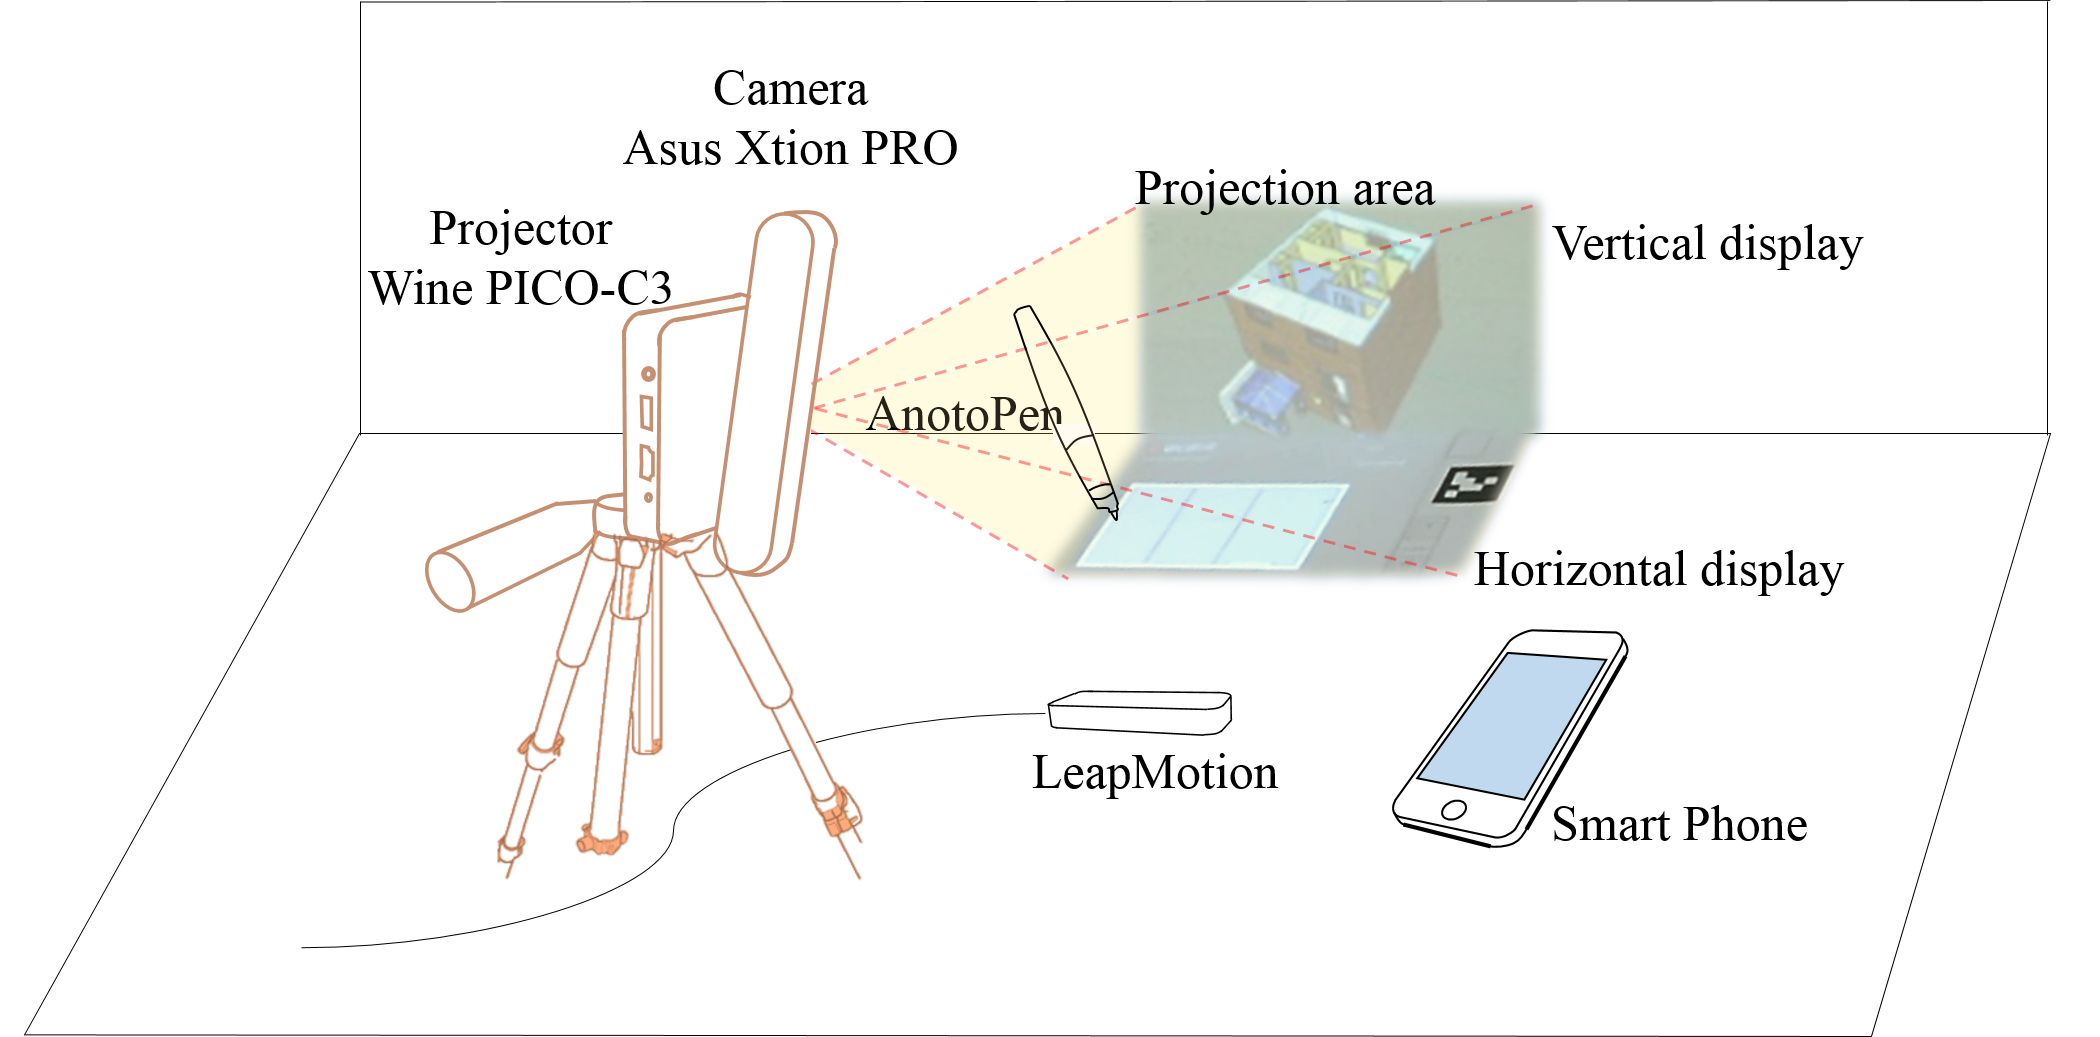
\includegraphics[width=\textwidth]{3-System/system_overview}
                \caption{System Components}
                \label{fig:port3dar}
        \end{subfigure}
        \\
        \begin{subfigure}[b]{1.0\columnwidth}
	        \centering
              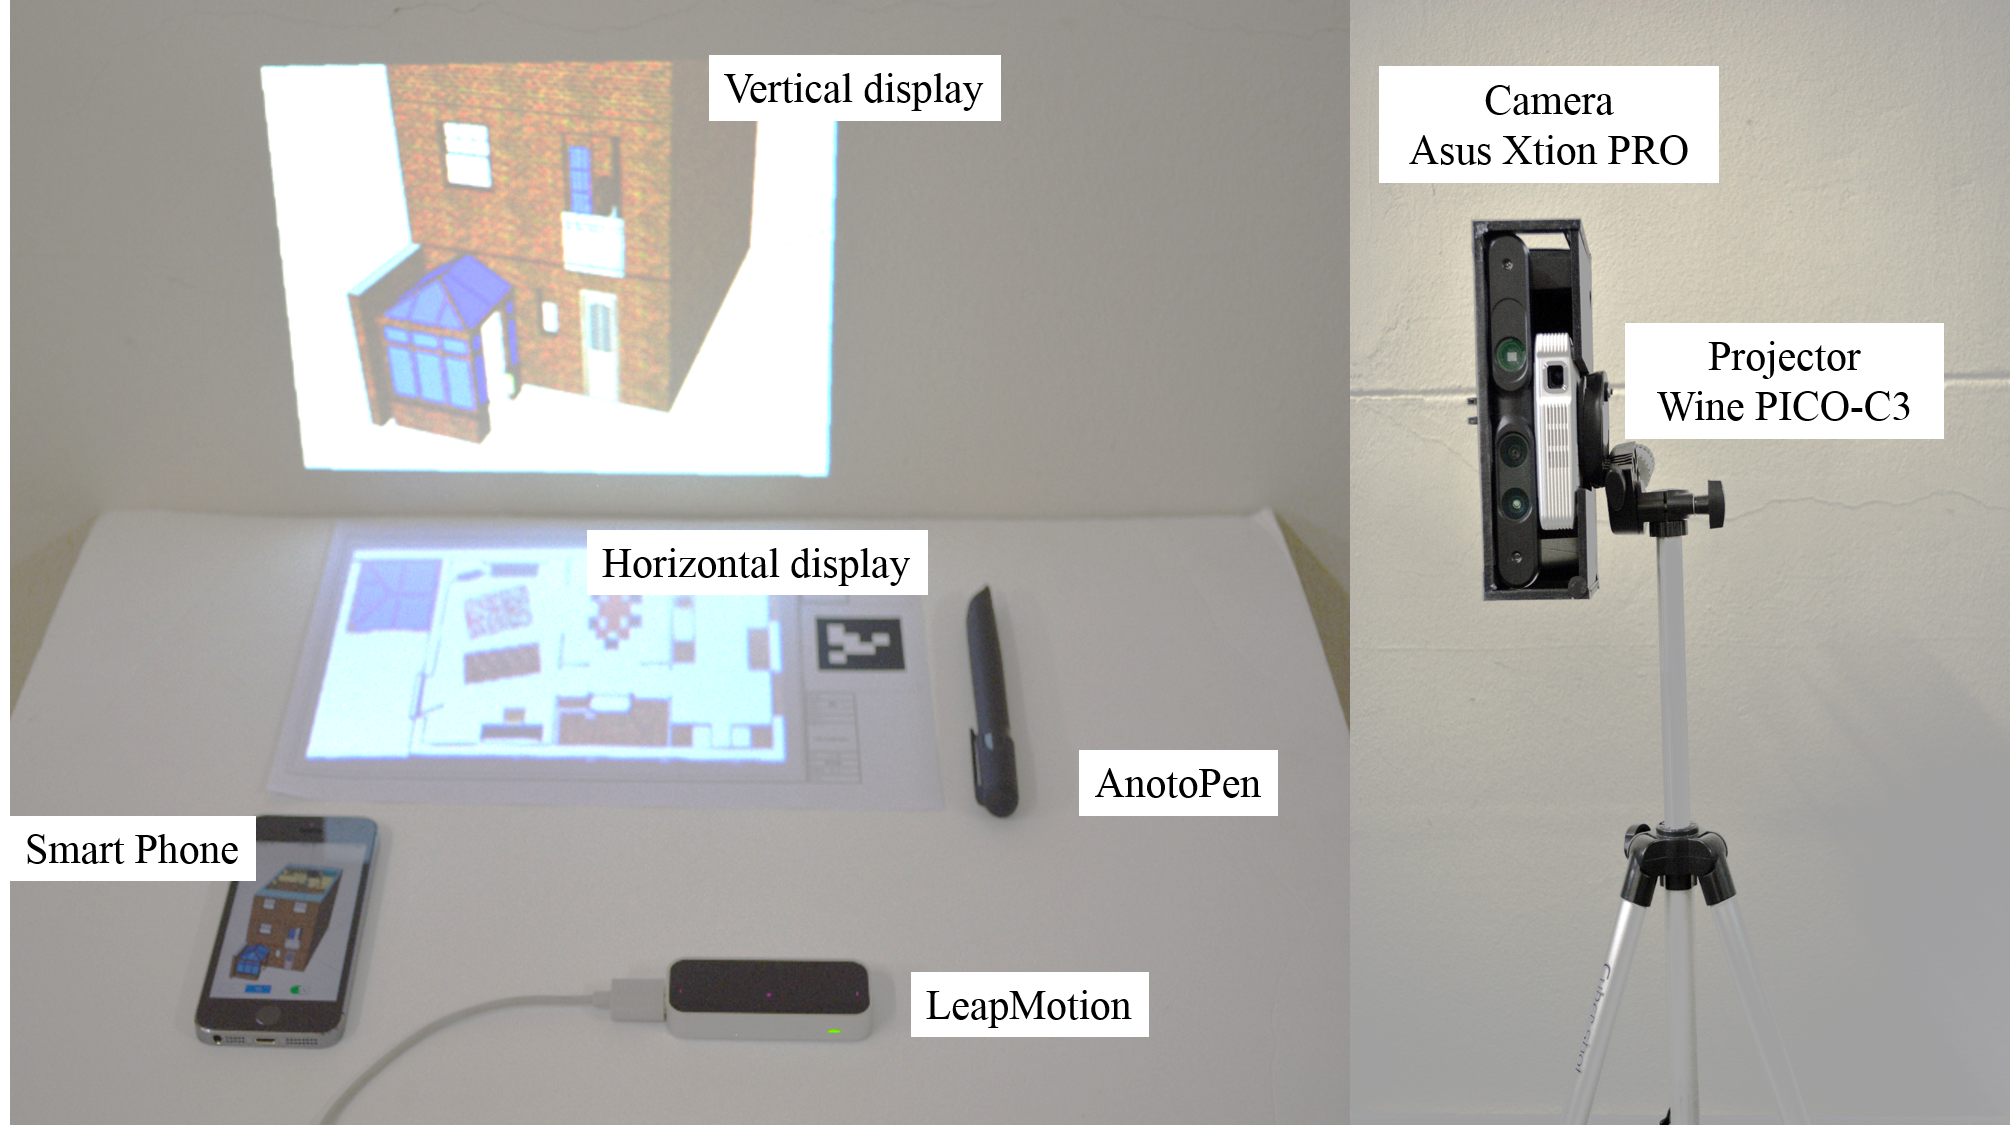
\includegraphics[width=\textwidth]{3-System/system}
              \caption{System Configuration}
              \label{fig:hardware}
        \end{subfigure}%
	\caption{Proposed Interactive 3D Smart Space System}
    \label{fig:system}
\end{figure}
\subsection{System Overview}

시스템 구조는 \ref{fig:overview}와 같이 User Interaction Layer, Construction Data Process Layer, Construction Data Storage Layer로 구분된다. User Interaction Layer에서는 사용자가 Vertical/Horizontal Display에 대히여 Hand, Pen 등을 이용하여 직접적인 제어가 가능하며, 실시간 Display에 대한 상태 확인이 가능하다. 또한 모바일 Device에서 센서 및 터치 기반의 상호작용은 인식하며 이를 처리한 결과를 모바일 디스플레이에 보여주는 기능을 담당한다. Construction Data Process Layer는 사용자의 제어를 입력받아 건축 모델에 반영하고 이 결과를 Vertical/Horizontal Display나 Mobile Display에 실시간 반영하는 역할을 수행한다. 마지막으로 Construction Data storage Layer는 수정되는 3D Model, Floor Plane와 같은 건축 정보를 관리한다.
%% 번역 원본
% As in Figure \ref{fig:overview}, the system consists of a \textit{User Interaction Layer}, a \textit{Construction Data Process Layer}, and a \textit{Construction Data Storage Layer}. In the \textit{User Interaction Layer}, the user can use a hand, pen, etc. to directly control the vertical/horizontal display and can also check the status of the display in real-time. Interactions based on touch or a sensor on a mobile device are recognized and the results are managed via functions shown on the mobile display. The \textit{Construction Data Process Layer} is controlled by user input, which is reflected in the construction model. This layer reflects these results on the vertical/horizontal display or mobile display in real-time. Finally, the \textit{Construction Data Storage Layer} manages construction information such as modified 3D models and floor plans.
%% 번역 결과
% As shown in Figure \ref{fig:overview}, the system consists of user interaction, construction data process, and construction data storage layers. In the user interaction layer, the user can use a hand, pen, or similar device to control the vertical/horizontal display directly and can also check the status of the display in real time. Interactions based on touch on a mobile-device sensor are recognized, and the results are managed using functions shown on the mobile display. The construction data process layer is controlled by user input, which is reflected in the construction model. This layer reflects these results on the vertical/horizontal display or mobile display in real time. Finally, the construction data storage layer manages construction information, such as modified 3D models and floor plans.

\subsection{Interactive 3D Smart Space}

제안하는 Interactive 3D Smart Space 시스템은 기존의 시스템과 달리 하나의 Portable Device에서 Vertical Display와 Horizontal Display를 동시에 제공하며 이를 통하여 3차원 정보를 제공하고 향상된 NUI 기술과 펜을 이용하여 이를 제어하도록 설계하였다\ref{fig:port3dar}. 이를 위하여 전체 시스템의 구성은 크게 Interaction과 Multi-view Display로 나눠볼수 있다. Interaction에서 사용되는 인식 디바이스는 카메라, 립모션, 펜 으로 나눠진다. 카메라는 Horizontal display의 마커를 인식하고 사용자의 터치를 인식하는데 사용되고, Leap Motion은 사용자의 3D 제스처/포스처를 인식하여 Vertical display를 제어하는데 사용된다. 또한 펜은 Horizontal 영역의 사용자 스케치를 인식하여 Vertical display를 조작/갱신하는데 사용된다. 이를 위하여 \cite{wobbrock_gestures_2007} 기반의 간단한 스케치 인식 기술을 적용하였다. 펜은 OSC(Open Sound Control) 프로토콜\cite {wright_open_1997}을 이용하여 서버와 통신하며 데이터를 전송한다. 펜 뿐만 아니라 카메라, 립모션 역시 제어하는 display에서 갱신된 정보를 각각 다른 display에 갱신한다. 연구에서 적용된 하드웨어의 구성품은  [Figure \ref {fig:hardware}] 같다.
%% 번역 원본
% Unlike previous systems, the proposed Interactive 3D Smart Space offers vertical and horizontal display simultaneously on the same device while providing 3D information through this; it is designed so that this information can be controlled using improved NUI technology and a pen (Figure \ref{fig:port3dar}). The overall system structure can be broadly divided into interaction and multi-view display for this. The recognition devices used in interactions are a depth camera, \textit{Leap Motion}, and a pen. The camera recognizes the horizontal display marker and is used through recognition of a user's touch, and \textit{Leap Motion} recognizes a user's 3D gestures/postures for use in controlling the vertical display. The pen is used to manipulate and modify the vertical display through recognizing a user's sketches in a horizontal field. For this, simple sketch recognition technology based on \cite{wobbrock_gestures_2007} is used. The pen uses OSC (Open Sound Control) protocol\cite{wright_open_1997} to communicate with the server and transmit data. Updated information is updated on each display as well as the original display controlled by the pen, camera or \textit{Leap Motion}. %The hardware structure used in the study is as in Figure \ref{fig:hardware}.

% In contrast to previous systems, the proposed interactive 3D smart space offers vertical and horizontal display simultaneously on the same device, while providing 3D information through it; it is designed so that this information can be controlled using improved NUI technology and a pen (see Figure \ref{fig:port3dar}). The overall system structure can be divided broadly into an interaction and multi-view display for this purpose. The recognition devices used in interactions are a depth camera, Leap Motion, and a pen. The camera recognizes the horizontal display marker and is used through recognition of a user's touch, while Leap Motion recognizes a user's 3D gestures/postures for use in controlling the vertical display. The pen is used to manipulate and modify the vertical display through recognizing a user's sketches in a horizontal field. Simple sketch recognition technology based on \cite{wobbrock_gestures_2007} is used to accomplish this. The pen uses the Open Sound Control (OSC) protocol to communicate with the server and transmit data. Information is updated on each display, along with the original display controlled by the pen, camera, or Leap Motion.

\begin{comment}
\begin{figure}[!h]
	\centering
        \begin{subfigure}[b]{0.49\columnwidth}
	        \centering
                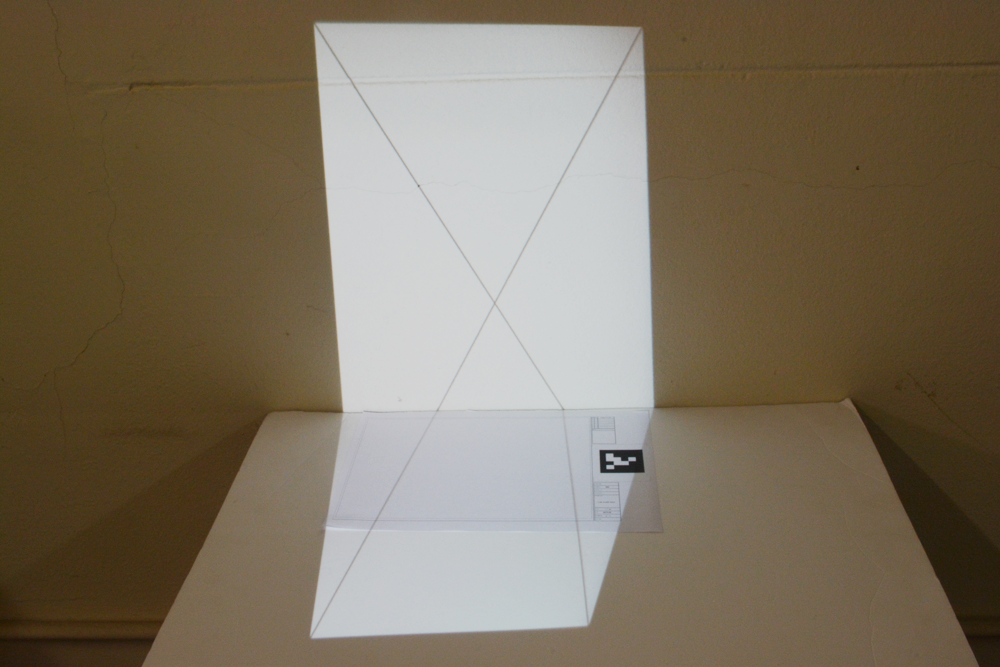
\includegraphics[width=\textwidth]{3-System/non_rectified}
                \caption{Non-rectified Planes}
                \label{fig:non-rectified}
        \end{subfigure}%
        \hfill
        \begin{subfigure}[b]{0.49\columnwidth}
            \centering
            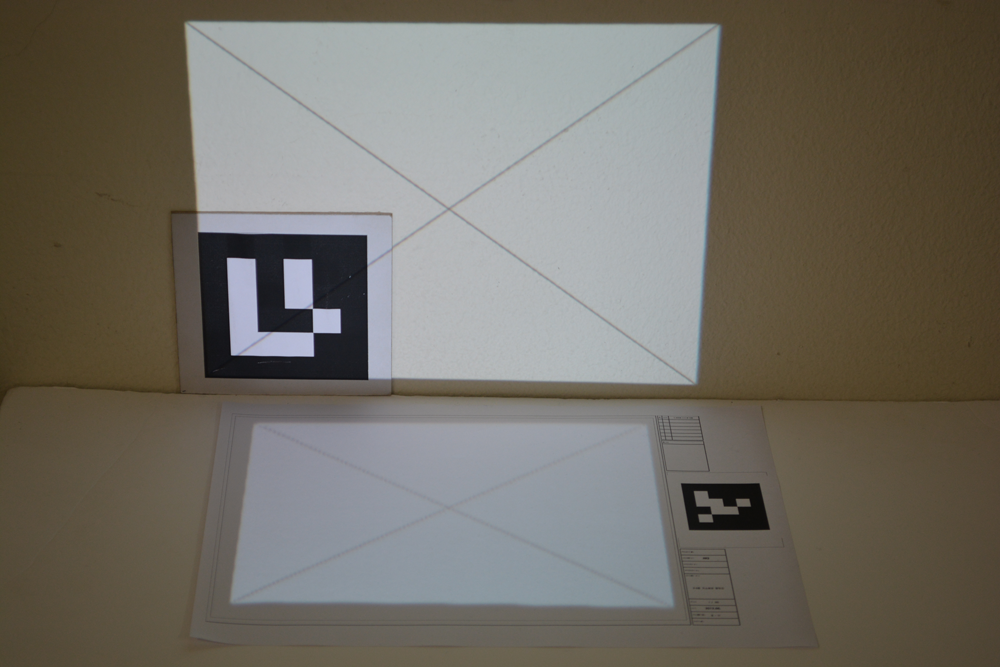
\includegraphics[width=\textwidth]{3-System/rectified}
                \caption{Marker-based Rectification}
                \label{fig:marker_rectify}
        \end{subfigure}
	\caption{Projection Plane Rectification}
    \label{fig:rectification}
\end{figure}
\end{comment}

% \begin{figure}[b!]
% \centering
% 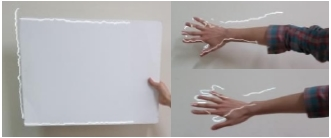
\includegraphics[width=1.0\columnwidth, height=3cm]{3-System/Calibration_result}
% \caption{Projector-Camera Calibration Result}
% \label{fig:calibration}
% \end{figure}

Multi-view Display는 인식 기기들의 제어로 갱신된 정보들이 실시간 업데이트 되며, 'L'-shape 벽면에 Vertical/Horizontal display를 각각 투영한다. 먼저 Vertical display는 3D Model이 투영된다. 이를 통해 사용자는 직관적으로 3차원 모델의 조작이 가능하다. Horizontal display에는 건축 도면이 display 되어 펜과 터치 기반의 상호작용이 가능하다. 이를 통하여 도면에서의 특정 entity의 정보를 질의하거나 도면에 직접 정보를 업데이트할 수 있도록 하였다. 일반적으로 벽면에 단순 투영을 하는 경우, projection plane과 projector 사이의 기하학적 위치 관계로 인하여, 화면의 모양이 일그러진다. 이를 보완하기 위하여 본 논문에서는 마커 기반의 Rectification 기술을 적용하였다. 
이를 위하여 먼저 Preliminary process로써 OpenCV의 Camera Calibration module \cite{opencv_2.4.8.0_documentation_camera_????}을 이용하여 프로젝터와 Depth 카메라 사이의 Calibration을 수행하였다. 이를 통하여 그림\ref{fig:calib_result}와 같이 Depth 카메라에서 인식된 World Coordinate에 정확하게 Projection 할 수 있다. 

%% 번역 원본
%Information controlled through recognition devices is instantly updated on the multi-view display while the vertical/horizontal displays are each projected on an L-shaped wall surface. First, the 3D model is projected on the Vertical Display. Through this, the user can intuitively operate the 3D model. The construction floor plans are displayed on the horizontal display and can be manipulated using pen- or touch-based interaction. Through this, specific entity information can be queried in the floor plans or information can be directly updated on them. For general projection on a regular wall, the screen's shape is distorted due to the geometric relationship between the projection plane and projector. In this paper, rectification technology based on markers was used to solve this problem. The OpenCV's Camera Calibration Module\cite{opencv_2.4.8.0_documentation_camera_????} was used as a preliminary process to calibrate the projector and the depth camera. Thus, as in Figure \ref{fig:calibration}, accurate projection could be achieved on the world coordinates recognized by the depth camera.

%% 번역 결과
% Information controlled using recognition devices is updated instantly on the multi-view display, while the vertical/horizontal displays are each projected onto an L-shaped wall surface. First, the 3D model is projected on the vertical display. In this way, the user can operate the 3D model intuitively. The construction floor plans are displayed on the horizontal display and can be manipulated using pen- or touch-based interaction. In this way, specific entity information can be queried in the floor plans, or information can be updated on them directly. For general projection on a regular wall, the screen's shape is distorted as a result of the geometric relationship between the projection plane and projector. In this paper, rectification technology based on markers was used to solve this problem. OpenCV's camera calibration module was used as a preliminary process to calibrate the projector and the depth camera. Thus, accurate projection could be achieved on the world coordinates recognized by the depth camera.

\begin{comment}
\begin{figure}[!h]
	\centering
        \begin{subfigure}[b]{1.0\columnwidth}
	        \centering
                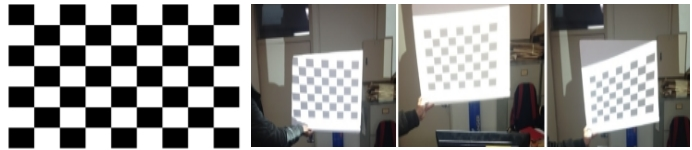
\includegraphics[width=\textwidth]{3-System/Calibration_pattern}
                \caption{Calibration pattern}
                \label{fig:calibration_pattern}
        \end{subfigure}%
        \\
        \begin{subfigure}[b]{1.0\columnwidth}
            \centering
            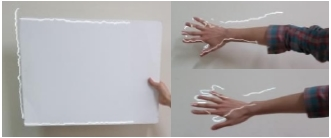
\includegraphics[width=\textwidth]{3-System/Calibration_result}
                \caption{Calibration result}
                \label{fig:calib_result}
        \end{subfigure}
	\caption{Projector-Camera Calibration}
    \label{fig:calibration}
\end{figure}
\end{comment}

이렇게 Calibration이 완료된 Projector-Depth Camera 시스템을 이용하여 'L'-shape 벽면의 평면 마커를 인식하도록 하였다 그림 \ref{fig:coordinate}와 같이 인식된 마커\cite{seo_enhancing_2011}의 좌표를 기준으로 프로젝션하는 영상의 좌표계를 설정하였다. 이를 통하여 영상의 프로젝션 왜곡을 보정하여 rectified 영상을 제공할 수 있다. 

%% 번역 원본
% In this way, using a calibrated projector-depth camera system, surface markers for an L-shaped wall surface were recognized(Figure \ref{fig:coordinate}). As in Figure \ref{fig:coordinate}, the coordinates of the recognized marker \cite{seo_enhancing_2011} were set to a frame of reference for a projected video. This corrected the video's projection distortion and allowed for a rectified video. 

%% 번역 결과
% Surface markers for an L-shaped wall surface were recognized in this way, using a calibrated projector-depth camera system (see Figure \ref{fig:coordinate}). As shown in Figure \ref{fig:coordinate}, the coordinates of the recognized marker were set to a frame of reference for a projected video. This corrected the video's projection distortion and allowed for a rectified video.

\begin{figure}[t!]
\centering
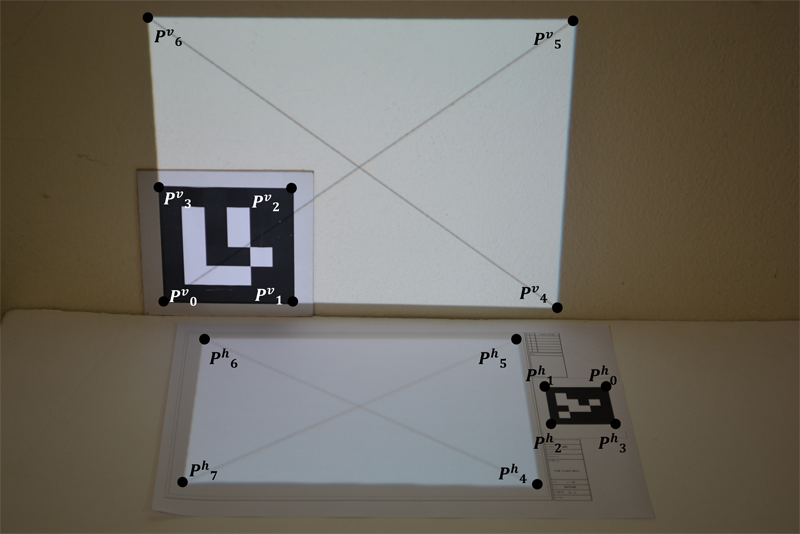
\includegraphics[width=0.8\columnwidth, height=4.2cm]{3-System/coordinates}
\caption{Coordinate Systems}
\label{fig:coordinate}
\end{figure}


\subsection{Personal Mobile Workspace}

\begin{figure}[!b]
\centering
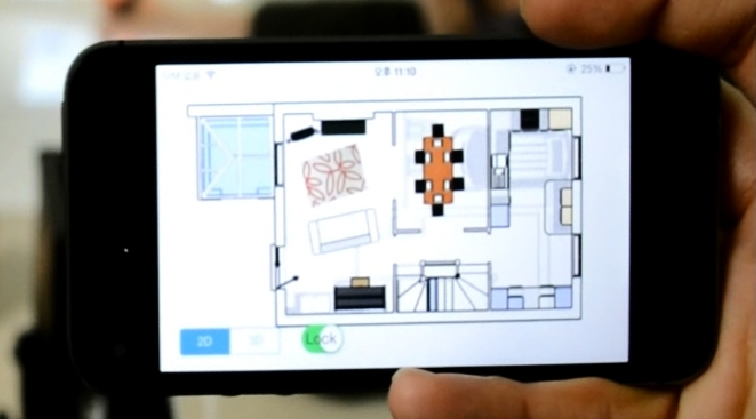
\includegraphics[width=1.0\columnwidth, height=4cm]{3-System/2d}
\caption{Personal Mobile Workspace}
\label{fig:pmw}
\end{figure}

\begin{figure*}[t!]
    \centering
        \begin{subfigure}[b]{0.32\textwidth}
            \centering
                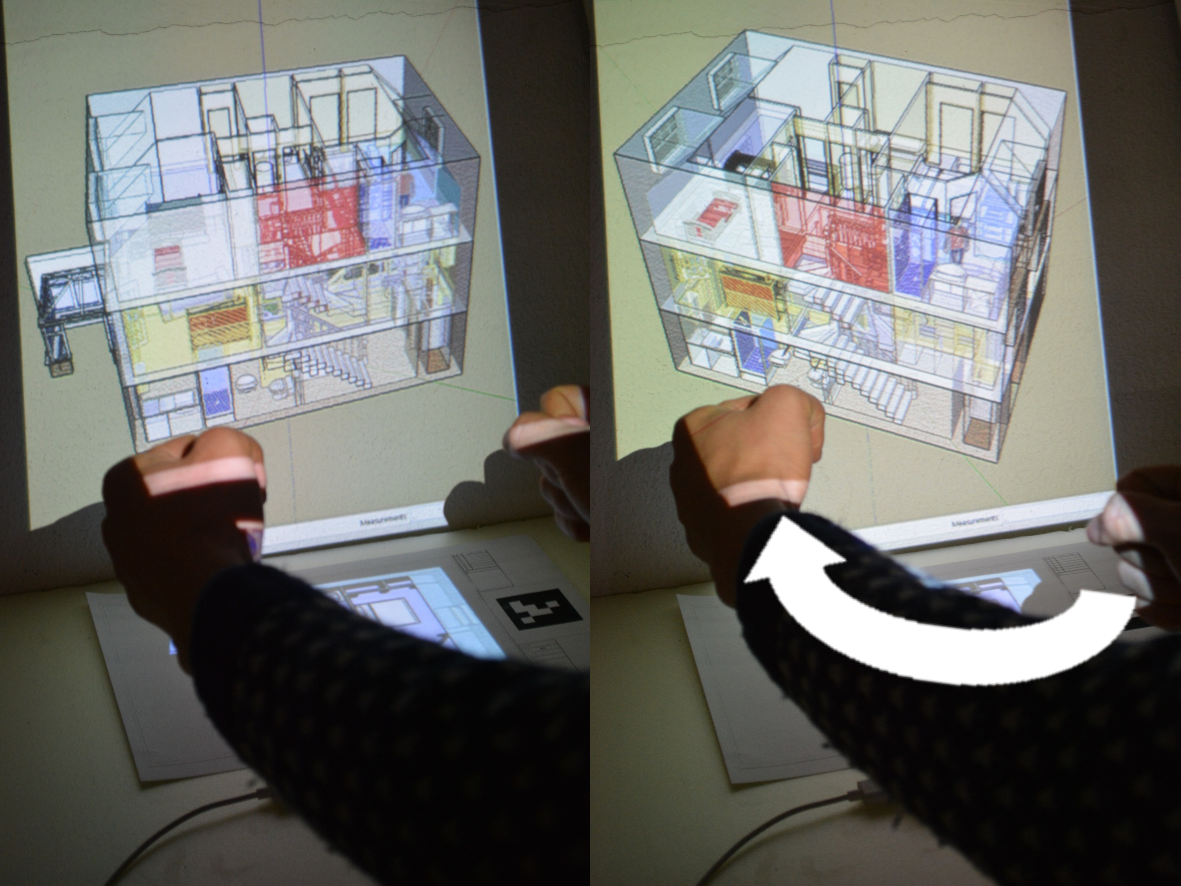
\includegraphics[width=\textwidth, height=3.5cm]{4-Interaction_Design/3d_rotation_1}
                \caption{Rotating the Model}
                \label{fig:rotate}
        \end{subfigure}%
        \hfill
        \begin{subfigure}[b]{0.32\textwidth}
            \centering
            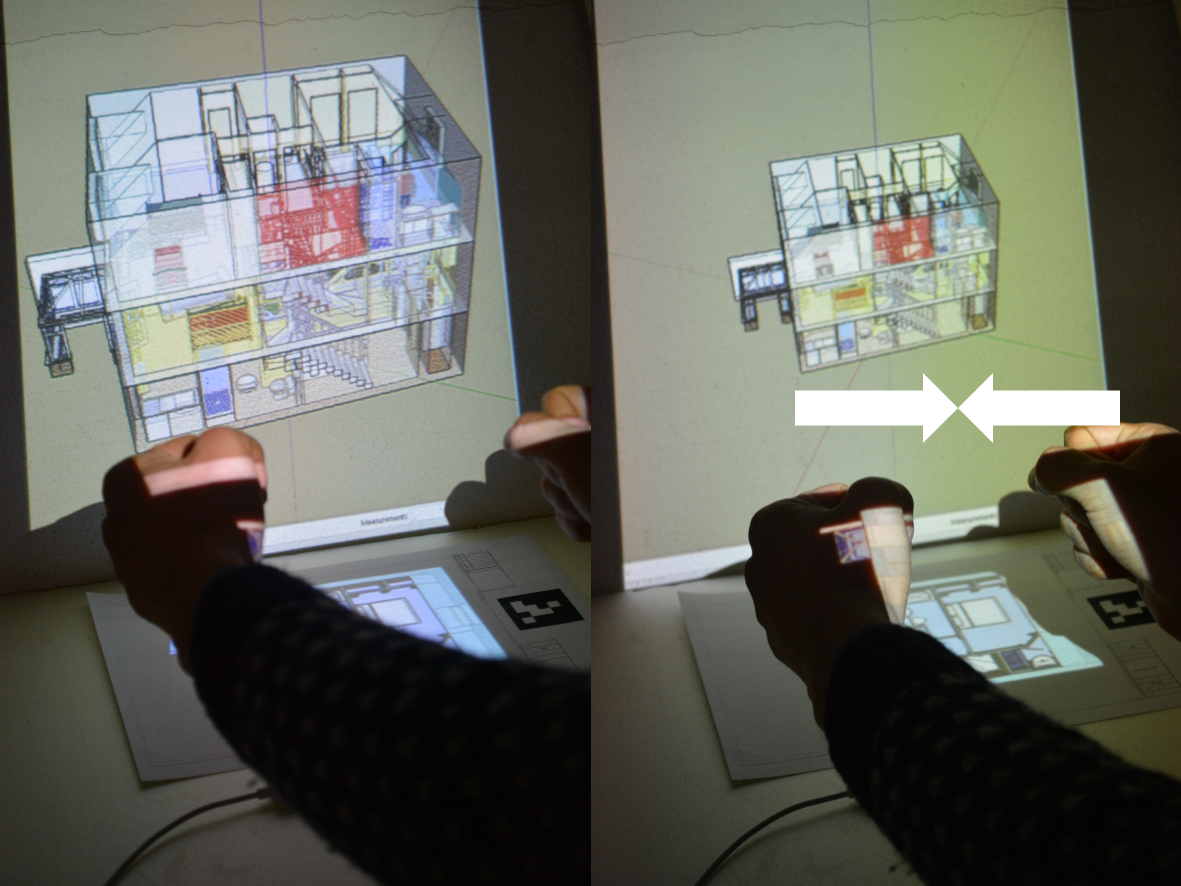
\includegraphics[width=\textwidth, height=3.5cm]{4-Interaction_Design/3d_scale}
                \caption{Scaling by Two Hand Gesture}
                \label{fig:scale_two_hand}
        \end{subfigure}
        \hfill
        \begin{subfigure}[b]{0.32\textwidth}
            \centering
            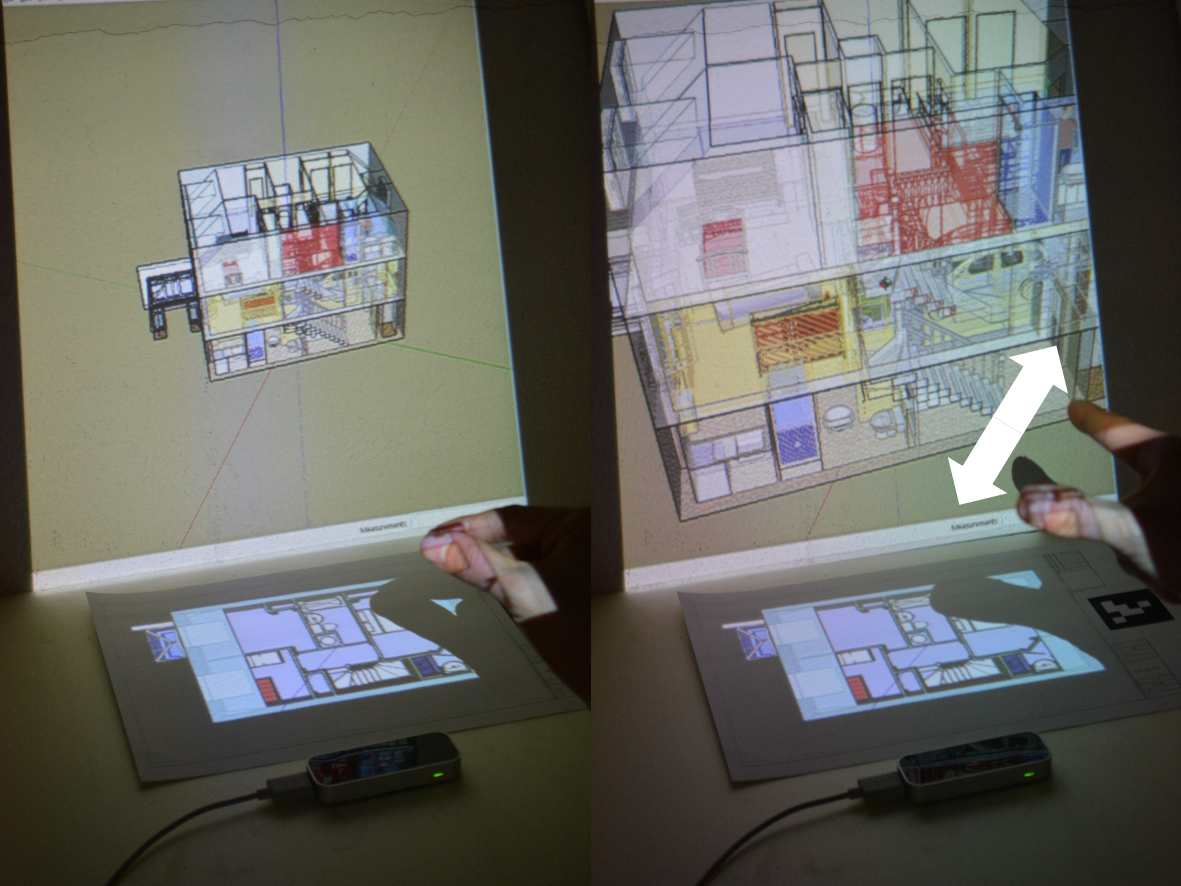
\includegraphics[width=\textwidth, height=3.5cm]{4-Interaction_Design/3d_scale_pinch}
                \caption{Scaling by One Hand Gesture}
                \label{fig:scale_pinch}
        \end{subfigure}
    \caption{3D model manipulation}
    \label{fig:3d_mani}
\end{figure*}

작업 도중에 건축 정보에 실시간으로 접근하기 위하여 모바일 폰을 이용하여 모델 정보에 접근하도록 하였다. 협업 환경인 Interactive 3D Smart Space의 정보를 현장에서 곧바로 접근하여 확인하고, 이를 수정하여 실시간으로 Shared Workspace에 업데이트할 수 있다. 이를 위하여 \ref{fig:pmw}에서 보는 것과 같이 2-dimension 모드와 3-dimension 모드를 선택할 수 있도록 하였다. 이를 통하여 2차원 floor plan이나 3차원 모델을 손가락으로 확대/축소, 회전하여 내용을 확인하거나 터치하여 entity의 정보를 확인하고, Drag하여 Entity의 위치를 수정할 수 있다. 또한, 작업 전 회의 등의 경우에 Shared Workspace의 Contents를 모바일 폰을 이용하여 Manipulation 함으로써 Shared Workspace의 제한된 공간의 한계를 해결할 수 있도록 하였다. 또한, 작업 도중에 임시로 모델의 정보를 확인하고 조작할 수 있도록 \ref{fig:pmw}와 같이 Synchoronized Lock 버튼을 추가함으로써 개인 작업 환경의 독립성을 제공하였다. 

%% 번역 원본
% A mobile phone is used to access model information on the job on-the-fly. Interactive 3D Smart Space information in a cooperative environment can be immediately accessed and checked on-site, and modified information can be immediately updated on a Shared Workspace. As shown in Figure \ref{fig:pmw}, 2-dimensional mode or 3-dimensional mode can be selected for this. Through this, a 2D Floor Plan or 3D Model can be expanded/contracted or rotated with the fingers to check the information and can be touched to check entity information or dragged to modify entity location. As well, Shared Workspace contents can be used and manipulated on mobile phones in meetings before work so that the limitations of a Shared Workspace can be overcome. As in Figure \ref{fig:pmw}, temporary model information can be checked and manipulated on the job, and the addition of a \textit{Synchronized Lock} button provides independence in an individual work environment.

%% 번역 결과
% A mobile device is used to access model information on the job on the fly. Interactive 3D smart space information in a cooperative environment can be accessed immediately and checked on site, and modified information can be updated immediately on a shared workspace. As shown in Figure \ref{fig:pmw}, either 2D or 3D mode can be selected for this. In this way, a 2D floor plan or 3D model can be expanded, contracted, or rotated with the fingers to check the information and can be touched to check entity information or dragged to modify entity location. In addition, shared workspace contents can be used and manipulated on mobile devices in meetings before work, overcoming the limitations of a shared workspace. As shown in Figure \ref{fig:pmw}, temporary model information can be checked and manipulated on the job, and a synchronized lock button provides independence in an individual work environment.

% 한글버전
%제안하는 시스템은 Shared Workspace를 위한 Interactive 3D Smart Space 기술과 이러한 기술과 연결되어 작업 중에 실시간으로 활용 가능한 Mobile personal workspace 기술로 이루어진다. Interactive 3D Smart Space 기술은 여러명의 작업자가 2D Floor Plan과 3D 건축 모델을 상호작용할 수 있도록 NUI 기술과 펜 입력을 이용하여 편리한 상호작용을 제공한다. 이렇게 정리된 건축 모델 정보를 실제 작업자가 작업 도중에 정보에 접근하고 업데이트하며 커뮤니케이션하기 위하여 모바일 폰을 이용하여 상호작용하도록 하였다.

\subsection{System Overview}

시스템 구조는 \ref{fig:overview}와 같이 User Interaction Layer, Construction Data Process Layer, Construction Data Storage Layer로 구분된다. User Interaction Layer에서는 사용자가 Vertical/Horizontal Display에 대히여 Hand, Pen 등을 이용하여 직접적인 제어가 가능하며, 실시간 Display에 대한 상태 확인이 가능하다. 또한 모바일 Device에서 센서 및 터치 기반의 상호작용은 인식하며 이를 처리한 결과를 모바일 디스플레이에 보여주는 기능을 담당한다. Construction Data Process Layer는 사용자의 제어를 입력받아 건축 모델에 반영하고 이 결과를 Vertical/Horizontal Display나 Mobile Display에 실시간 반영하는 역할을 수행한다. 마지막으로 Construction Data storage Layer는 수정되는 3D Model, Floor Plane와 같은 건축 정보를 관리한다.

\subsection{Interactive 3D Smart Space}
\begin{figure}[!ht]
	\centering
        \begin{subfigure}[b]{1.0\columnwidth}
            \centering
            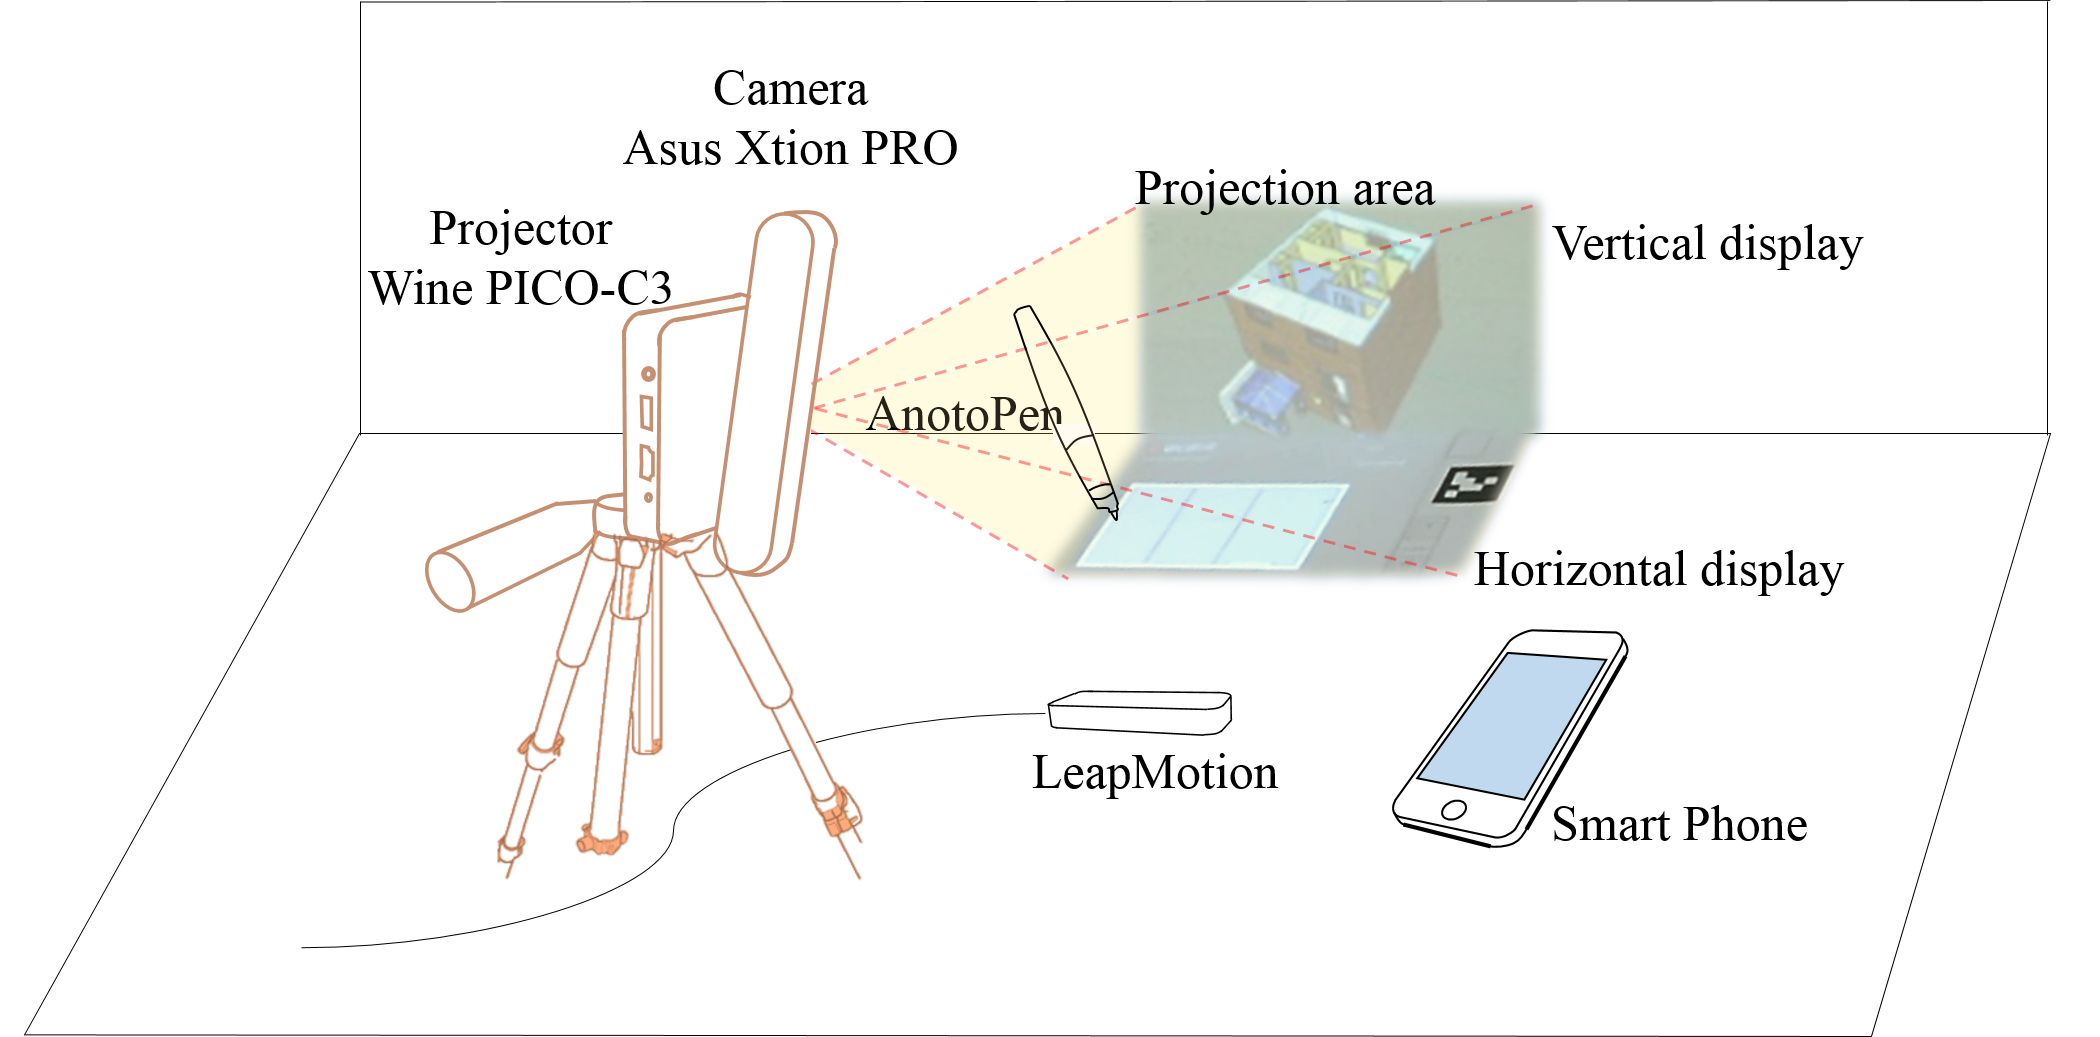
\includegraphics[width=\textwidth]{3-System/system_overview}
                \caption{System Components}
                \label{fig:port3dar}
        \end{subfigure}
        \\
        \begin{subfigure}[b]{1.0\columnwidth}
	        \centering
              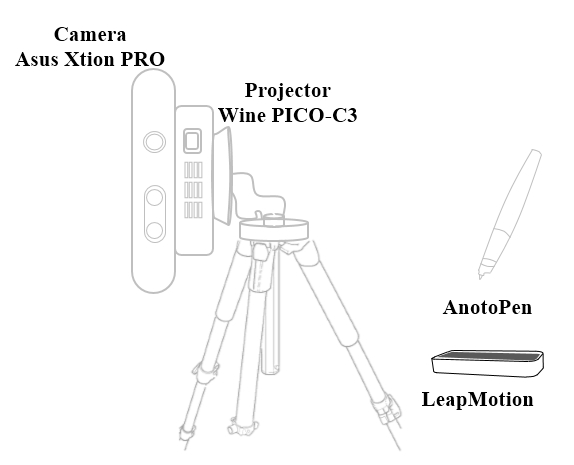
\includegraphics[width=0.7\columnwidth]{3-System/Hardware}
              \caption{System Hardware}
              \label{fig:hardware}
        \end{subfigure}%
	\caption{Proposed Interactive 3D Smart Space System}
    \label{fig:system}
\end{figure}
제안하는 Interactive 3D Smart Space 시스템은 기존의 시스템과 달리 하나의 Portable Device에서 Vertical Display와 Horizontal Display를 동시에 제공하며 이를 통하여 3차원 정보를 제공하고 향상된 NUI 기술과 펜을 이용하여 이를 제어하도록 설계하였다\ref{fig:port3dar}. 이를 위하여 전체 시스템의 구성은 크게 Interaction과 Multi-view Display로 나눠볼수 있다. Interaction에서 사용되는 인식 디바이스는 카메라, 립모션, 펜 으로 나눠진다. 카메라는 Horizontal display의 마커를 인식하고 사용자의 터치를 인식하는데 사용되고, Leap Motion은 사용자의 3D 제스처/포스처를 인식하여 Vertical display를 제어하는데 사용된다. 또한 펜은 Horizontal 영역의 사용자 스케치를 인식하여 Vertical display를 조작/갱신하는데 사용된다. 이를 위하여 \cite{wobbrock_gestures_2007} 기반의 간단한 스케치 인식 기술을 적용하였다. 펜은 OSC(Open Sound Control) 프로토콜\cite {wright_open_1997}을 이용하여 서버와 통신하며 데이터를 전송한다. 펜 뿐만 아니라 카메라, 립모션 역시 제어하는 display에서 갱신된 정보를 각각 다른 display에 갱신한다. 연구에서 적용된 하드웨어의 구성품은  [Figure \ref {fig:hardware}] 같다.



\begin{figure}[!h]
	\centering
        \begin{subfigure}[b]{1.0\columnwidth}
	        \centering
                \includegraphics[width=\textwidth]{image_upload}
                \caption{Non-rectified Planes}
                \label{fig:non-rectified}
        \end{subfigure}%
        \\
        \begin{subfigure}[b]{1.0\columnwidth}
            \centering
            \includegraphics[width=\textwidth]{image_upload}
                \caption{Marker-based Rectification}
                \label{fig:marker_rectify}
        \end{subfigure}
	\caption{Projection Plane Rectification}
    \label{fig:rectification}
\end{figure}


Multi-view Display는 인식 기기들의 제어로 갱신된 정보들이 실시간 업데이트 되며, 'L'-shape 벽면에 Vertical/Horizontal display를 각각 투영한다. 먼저 Vertical display는 3D Model이 투영된다. 이를 통해 사용자는 직관적으로 3차원 모델의 조작이 가능하다. Horizontal display에는 건축 도면이 display 되어 펜과 터치 기반의 상호작용이 가능하다. 이를 통하여 도면에서의 특정 entity의 정보를 질의하거나 도면에 직접 정보를 업데이트할 수 있도록 하였다. 일반적으로 벽면에 단순 투영을 하는 경우, projection plane과 projector 사이의 기하학적 위치 관계로 인하여, \ref{fig:non-rectified}와 같이 화면의 모양이 일그러진다. 이를 보완하기 위하여 본 논문에서는 마커 기반의 Rectification 기술을 적용하였다. 
이를 위하여 먼저 Preliminary process로써 OpenCV의 Camera Calibration module \cite{opencv_2.4.8.0_documentation_camera_????}을 이용하여 프로젝터와 Depth 카메라 사이의 Calibration을 수행하였다\ref{fig:calibration}. 이를 통하여 그림\ref{fig:calib_result}와 같이 Depth 카메라에서 인식된 World Coordinate에 정확하게 Projection 할 수 있다. 

\begin{figure}[!h]
	\centering
        \begin{subfigure}[b]{1.0\columnwidth}
	        \centering
                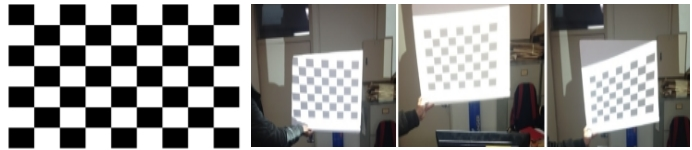
\includegraphics[width=\textwidth]{3-System/Calibration_pattern}
                \caption{Calibration pattern}
                \label{fig:calibration_pattern}
        \end{subfigure}%
        \\
        \begin{subfigure}[b]{1.0\columnwidth}
            \centering
            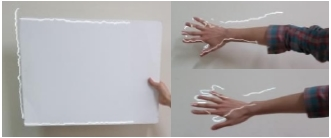
\includegraphics[width=\textwidth]{3-System/Calibration_result}
                \caption{Calibration result}
                \label{fig:calib_result}
        \end{subfigure}
	\caption{Projector-Camera Calibration}
    \label{fig:calibration}
\end{figure}

이렇게 Calibration이 완료된 Projector-Depth Camera 시스템을 이용하여 'L'-shape 벽면의 평면 마커를 인식하도록 하였다\ref{fig:marker_rectify} 그림 \ref{fig:coordinate}와 같이 인식된 마커\cite{seo_enhancing_2011}의 좌표를 기준으로 프로젝션하는 영상의 좌표계를 설정하였다. 이를 통하여 영상의 프로젝션 왜곡을 보정하여 rectified 영상을 제공할 수 있다. 
\begin{figure}[!h]
\centering
\includegraphics[width=0.7\columnwidth]{3-System/coordinate_systems}
\caption{Coordinate systems}
\label{fig:coordinate}
\end{figure}


\subsection{Personal Mobile Workspace}
작업 도중에 건축 정보에 실시간으로 접근하기 위하여 모바일 폰을 이용하여 모델 정보에 접근하도록 하였다. 협업 환경인 Interactive 3D Smart Space의 정보를 현장에서 곧바로 접근하여 확인하고, 이를 수정하여 실시간으로 Shared Workspace에 업데이트할 수 있다. 이를 위하여 \ref{fig:pmw}에서 보는 것과 같이 2-dimension 모드와 3-dimension 모드를 선택할 수 있도록 하였다. 이를 통하여 2차원 floor plan이나 3차원 모델을 손가락으로 확대/축소, 회전하여 내용을 확인하거나 터치하여 entity의 정보를 확인하고, Drag하여 Entity의 위치를 수정할 수 있다. 또한, 작업 전 회의 등의 경우에 Shared Workspace의 Contents를 모바일 폰을 이용하여 Manipulation 함으로써 Shared Workspace의 제한된 공간의 한계를 해결할 수 있도록 하였다\textcolor{red}{폰 움직여 3차원 manipulation 사진 추가}. 또한, 작업 도중에 임시로 모델의 정보를 확인하고 조작할 수 있도록 \ref{fig:pmw}와 같이 Synchoronized Lock 버튼을 추가함으로써 개인 작업 환경의 독립성을 제공하였다. 
\begin{figure}[!h]
\centering
\includegraphics[width=0.7\columnwidth]{image_upload}
\caption{Personal Mobile Workspace}
\label{fig:pmw}
\end{figure}


% 영어버전
%The proposed system links Interactive 3D Smart Space technology for a Shared Workspace with this technology for a Mobile Personal Workspace that can be used in real-time on the job. Interactive 3D Smart Space technology uses NUI technology and pen input for convenient interactions to enable several workers to interact with the same 2D Floor Plan and 3D Model. Workers can view and update this organized construction model information while at work and mobile phones are used for interaction and communication. 

\subsection{System Overview}

